% !TEX program = xelatex
% Q1 standalone paper on the frozen chm.q1.v2.0 model.
% Data description: problem/readable/DATA_DESCRIPTION_VISIBLE.md only.
\documentclass[bwprint,withoutpreface]{gmcmthesis}
\hypersetup{hidelinks}
\usepackage{float}
\usepackage{siunitx}
\graphicspath{{figures/}{figures/chm/}}
\title{问题一：数据质量评价、指标冲突与领域配比建模}

\begin{document}
\maketitle
\begin{abstract}
针对题目附件 A 的质量信号和训练配比实验，本文建立逐文本与逐领域的质量代理，分析指标冲突，并构建 17 维配比到 13 个目标域交叉熵 Loss 的条件性决策模型。对 A1 的 51,230 条记录统一处理 22 个指标，按家族等权合成质量分数；冻结该规则后，对 A2/A3 全量扩展集及去重记录进行对照。以方向统一后的秩相关识别冲突，55 条显著负相关指标边在去重扩展集复现；采用综合质量与指标分歧的二维评价，标记需复核文本而不伪造人工质量真值。

对 A4+A5 的 512 个配方，本文逐目标拟合含 17 个主项与 10 个二元乘积项的交互代理。训练内嵌套五折比较中，交互模型在 13 个目标域的 RMSE 均低于线性 Ridge，目标域中位数分别为 0.4499 和 0.4921。A6--A11 用于同条件比较；这些组曾影响模型选择，不能视为全新盲测。在 A4 配方凸包内，采用 McCormick 松弛与空间分支定界计算等权、质量约束及最差域保护情景，四组浮点数值上下界间隙均小于 0.001。A12--A15 为估算外推表：交互代理与 10B、70B 估算 Loss 的排序相关中位数仅为 0.4915、0.3941，不能支持真实大模型的配方最优主张。最终答案是在明确权重、质量政策和支持范围内可复现的条件性配方决策。
\keywords{数据质量\quad 指标冲突\quad 领域配比\quad 交互回归\quad 多目标决策}
\end{abstract}
\maketoc
\clearpage

% Owner: chm. Rigorous Q1 restructure based only on visible problem/data description and current Attachment A results.
% Numeric evidence: outputs/chm/domain_quality.csv, outputs/chm/local_recheck_v1,
% outputs/chm/ablation_v1. Continuous mixture-scale transfer is intentionally excluded.
\section{问题一：数据质量评价与训练数据配比效应}
\label{sec:q1}

\subsection{问题分析与可识别性边界}

问题一包含两类由附件 A 直接支持的任务：一是利用 A1--A3 的 22 维质量信号评价七个语料域并分析指标冲突；二是利用 A4--A15 的 17 维训练配比与 13 个目标验证域交叉熵 Loss，分析训练配方与目标域 Loss 的关系。两类数据的域体系并不一一对应，因此本文分别建立 A 侧综合质量代理与逐目标域配比代理，再通过 A16 的映射类型和显式接口向后续问题传递结果，不人为补造跨附件数值关系。

A1 含 51,230 条质量记录；A2、A3 分别给出 arxiv 的 17,523 条和 github 的 203,752 条扩展记录。A4+A5 是 512 组 1M 配方及对应的 13 维 Loss；A6+A7、A8+A9、A10+A11 分别为 1M、60M、1B 检验组；A12--A15 在数据说明中明确属于 estimated/extrapolated，只用于压力测试。配比表和 Loss 表均按 \texttt{index} 一一对应。

需要特别限定的是，A4--A15 的配比表只给出 17 个比例，Loss 表只给出 13 个目标域 Loss；与这些配方实验相对应的训练数据量 $D$ 并未作为字段提供。模型规模 $1\mathrm{M}$、$60\mathrm{M}$、$1\mathrm{B}$ 仅由不同实验文件组标识。因此第一问可以检验“小模型配比代理在不同实验组上的排序是否保持”，但不能仅凭附件 A 识别连续的 $N$--$D$ 标度律，也不能把三个离散实验组拟合成普适的配比尺度衰减函数。基于这一可识别性边界，A6--A11 在本问中只承担冻结模型后的 held-out 验证，不再用于拟合额外的跨规模参数。

\subsection{A 侧综合质量代理}

\subsubsection{列表字段压缩与稳健标准化}

A1--A3 提供 22 个质量信号，其中 14 个为标量，8 个为列表字段。根据 SlimPajama-Meta-rater 公开数据卡\cite{metaraterdata}，二分类字段 \texttt{ad\_en} 与 \texttt{fluency\_en} 的两个元素为 logits，本文以 softmax 后的正类概率保留连续置信信息；四个 ModernBERT 字段是 $0$--$5$ 六等级 logits，以期望等级压缩；\texttt{qurater} 的四个评分分量取均值；\texttt{fineweb\_edu} 取唯一元素。argmax 压缩保留为敏感性方案，而不与主方案混用。

计数型指标先作 $\log(1+x)$ 变换，DSIR 三项作 signed-log 变换。不同指标量纲和尾部分布差异较大，因此仅用 A1 估计中心与尺度，采用 median--MAD 稳健标准化：
\begin{equation}
z_{ij}
=
\operatorname{clip}\!\left(
\frac{x_{ij}-\operatorname{median}(x_j)}
{1.4826\,\operatorname{MAD}(x_j)},
-5,5
\right).
\label{eq:q1_robust_z}
\end{equation}
其中 $i$ 表示记录，$j$ 表示指标。A2、A3 复用 A1 的变换、中心和尺度，避免扩展集信息反向进入评分口径。

\subsubsection{指标方向的确定}

八个模型评分字段的语义可以由数据卡直接确定为“数值越大，目标质量属性越强”，因此其方向固定为正。将这八项稳健标准化值的可用项均值定义为语义锚点
\begin{equation}
A_i=\frac{1}{|\mathcal M_i|}\sum_{j\in\mathcal M_i}z_{ij},
\label{eq:q1_quality_anchor}
\end{equation}
其中 $\mathcal M_i$ 为记录 $i$ 上非缺失的模型评分字段集合。

对于其余 14 个统计型指标，数据本身并不给出统一的“越大越好/越小越好”真值，因此不依据字段名称主观设定符号，而是在 A1 的每个质量域 $d$ 内计算
\begin{equation}
\rho_{jd}
=
\rho_{\mathrm S}(z_{ij},A_i\mid i\in d),
\label{eq:q1_orientation_rho}
\end{equation}
并用 Fisher 变换汇总域内相关：
\begin{equation}
\bar z_j
=
\frac{\sum_{d}(n_{jd}-3)\operatorname{arctanh}(\rho_{jd})}
{\sum_d(n_{jd}-3)},
\qquad
\bar\rho_j=\tanh(\bar z_j).
\label{eq:q1_fisher_pool}
\end{equation}
指标方向取 $d_j=\operatorname{sgn}(\bar\rho_j)$，再令 $z^+_{ij}=d_jz_{ij}$。该步骤的含义仅是“将统计型指标与已知语义的模型评分锚点对齐”，并不能把锚点或其方向解释成客观质量真值。域间符号一致率及 leave-one-domain-out 方向稳定性同时保留为敏感性证据。

\subsubsection{综合代理的定义与边界}

题目附件没有提供样本级“真实质量”标签，因此质量标量不能由监督学习唯一识别。本文采用最小附加假设的分组等权复合指标：RPS/Natural、DSIR、model-based 三个指标家族先在组内对可用项等权，再在三组之间等权。对记录 $i$，令
\begin{equation}
G_{ig}
=
\frac{1}{|\mathcal J_{ig}|}
\sum_{j\in\mathcal J_{ig}}z^+_{ij},
\qquad
S_i=\frac{1}{3}\sum_{g\in\{\mathrm{RPS,DSIR,MODEL}\}}G_{ig},
\label{eq:q1_family_score}
\end{equation}
其中 $\mathcal J_{ig}$ 是记录 $i$ 在家族 $g$ 中的非缺失指标集合。进一步用 A1 全体记录的均值和标准差定义 A 侧综合质量代理
\begin{equation}
Q_{A,i}=\frac{S_i-\mu_{S,A1}}{\sigma_{S,A1}}.
\label{eq:q1_QA}
\end{equation}
式\eqref{eq:q1_family_score}--\eqref{eq:q1_QA}是透明的复合指标定义，而不是由附件识别出的唯一“真实质量函数”。分组等权的理由只是避免某个指标家族因字段数量更多而自动获得更大总权重，因此必须与 22 指标完全等权、列表 argmax 压缩和家族删除方案同时做敏感性检验。

域级主统计量采用 $Q_A$ 中位数；固定评分规则下的记录 bootstrap 给出条件区间。结果见表\ref{tab:q1_quality}。

\begin{table}[htbp]
\centering\small
\caption{A1 七个质量域的综合质量代理}
\label{tab:q1_quality}
\begin{tabular}{lrrl}
\toprule
质量域 & 样本数 & $Q_A$ 中位数 & 条件 95\% 区间 \\
\midrule
arxiv & 1419 & 2.6826 & [2.6518, 2.7084] \\
book & 171 & 2.7711 & [2.6735, 2.8086] \\
c4 & 10000 & $-0.2173$ & [$-0.2376$, $-0.1997$] \\
commoncrawl & 9640 & 0.5061 & [0.4923, 0.5224] \\
github & 10000 & $-0.5171$ & [$-0.5438$, $-0.4886$] \\
stackexchange & 10000 & 0.1874 & [0.1723, 0.2025] \\
wikipedia & 10000 & $-0.3759$ & [$-0.4003$, $-0.3473$] \\
\bottomrule
\end{tabular}
\end{table}

\begin{figure}[htbp]
\centering

\includegraphics[width=.84\linewidth]{q1_quality_domain_intervals.png}
\caption{七域综合质量代理的中位数与条件区间。横轴为 A1 内部标准化坐标，不是附件 B 的原生 $Q_{\mathrm{score}}$。}
\label{fig:q1_quality}
\end{figure}

主方案与 argmax 压缩、22 指标完全等权方案的七域排名 Spearman 均为 0.9643，但分别发生 github/wikipedia 与 book/arxiv 的相邻次序交换。进一步删除 RPS 家族后，七域排名 Spearman 降至 0.8214，且 4 个域改变名次。因此图\ref{fig:q1_quality}中的窄 bootstrap 区间只量化固定评分规则下的记录抽样误差，不能替代评分规则不确定性。

\subsubsection{指标冲突与扩展集复核}

指标冲突不再引入额外的人造“冲突强度函数”，而直接使用标准的 Spearman 秩相关。对方向统一后的任意两指标 $j$、$r$，在质量域 $d$ 内计算
\begin{equation}
\rho_{jr,d}
=
\rho_{\mathrm S}(z^+_{ij},z^+_{ir}\mid i\in d).
\label{eq:q1_pair_spearman}
\end{equation}
若 $\rho_{jr,d}<0$，表示在该域中两指标对样本的相对排序方向相反；只有在多个域或扩展数据中重复出现时，才将其视为稳定的描述性冲突。当前尚未完成全部相关系数的区间估计和多重比较校正，因此论文不使用“显著冲突”这一表述。

A1 的 1419 条 arxiv 和 10000 条 github 记录均包含于对应扩展集，故 A2/A3 不能直接称为独立验证。剔除重叠后，另有 arxiv 16104 条和 github 193752 条记录可用于复核。冻结 A1 的全部处理参数后，非重叠记录的 $Q_A$ 中位数分别为 2.7146 和 $-0.5363$，与 A1 的 2.6826 和 $-0.5171$ 接近。代表性负相关见表\ref{tab:q1_conflict}。

\begin{table}[htbp]
\centering\small
\caption{A2/A3 非重叠记录中的代表性指标冲突}
\label{tab:q1_conflict}
\begin{tabular}{llr}
\toprule
域 & 方向统一后的指标对（简写） & Spearman \\
\midrule
arxiv & 大写字母行占比 / 终止标点行占比 & $-0.8195$ \\
arxiv & DSIR wiki / 非字母词占比 & $-0.6303$ \\
github & 大写字母行占比 / 终止标点行占比 & $-0.7442$ \\
github & 词汇唯一率 / 高频三元字符占比 & $-0.4902$ \\
\bottomrule
\end{tabular}
\end{table}

\subsection{17 域配比与目标域 Loss 的关系}

\subsubsection{组成约束与逐目标域 Ridge}

A4 的每一行是 17 个训练域比例。由于原始 CSV 的三位小数舍入会使行和轻微偏离 1，建模前按行归一化，记
\begin{equation}
\boldsymbol p_i=(p_{i1},\ldots,p_{i,17})^\top,
\qquad
p_{ij}\ge 0,\qquad
\boldsymbol 1^\top\boldsymbol p_i=1.
\label{eq:q1_simplex}
\end{equation}
A5 提供同一 \texttt{index} 下的 13 个目标验证域 Loss。不同目标域的 Loss 水平和波动尺度不同，因此不把 13 个原始 Loss 先求算术平均，而对每个目标域 $k$ 单独拟合。

以 A4 归一化配方的均值为参考配方
\begin{equation}
\boldsymbol p_{\mathrm{ref}}
=
\frac{1}{512}\sum_{i=1}^{512}\boldsymbol p_i,
\label{eq:q1_pref}
\end{equation}
则 $\boldsymbol q_i=\boldsymbol p_i-\boldsymbol p_{\mathrm{ref}}$ 满足 $\boldsymbol 1^\top\boldsymbol q_i=0$。在该 16 维单纯形切空间内，使用 L2 正则线性回归\cite{regmix2025}：
\begin{equation}
(\widehat\alpha_k,\widehat{\boldsymbol\beta}_k)
=
\arg\min_{\alpha,\boldsymbol\beta}
\left\{
\sum_{i=1}^{512}
\left[
L_{ik}-\alpha-\boldsymbol\beta^\top
(\boldsymbol p_i-\boldsymbol p_{\mathrm{ref}})
\right]^2
+
\lambda_k\|\boldsymbol\beta\|_2^2
\right\},
\quad
\text{s.t. }\boldsymbol 1^\top\boldsymbol\beta=0.
\label{eq:q1_constrained_ridge}
\end{equation}
$\lambda_k$ 仅在 A4+A5 的 512 条记录内通过 5 折交叉验证，从既定网格中选择；A6--A15 均不参与调参。

约束 $\boldsymbol 1^\top\boldsymbol\beta=0$ 不是额外经验假设，而是组成数据的规范化表示。因为对任意常数 $c$，
\[
(\boldsymbol\beta+c\boldsymbol 1)^\top
(\boldsymbol p-\boldsymbol p_{\mathrm{ref}})
=
\boldsymbol\beta^\top
(\boldsymbol p-\boldsymbol p_{\mathrm{ref}}),
\]
故只有系数之间的对比可识别；零和约束选取其中唯一的最小范数表示。当前实现先在精确归一化单纯形上拟合 Ridge，再将等价系数表示平移为零和形式，预测值保持不变。

由式\eqref{eq:q1_constrained_ridge}得到 1M 配比代理
\begin{equation}
\widehat L_{k,1M}(\boldsymbol p)
=
\widehat\alpha_k
+
\widehat{\boldsymbol\beta}_k^\top
(\boldsymbol p-\boldsymbol p_{\mathrm{ref}}).
\label{eq:q1_1m_surrogate}
\end{equation}
定义相对参考配方的配比效应
\begin{equation}
m_k(\boldsymbol p)
=
\widehat L_{k,1M}(\boldsymbol p)
-
\widehat L_{k,1M}(\boldsymbol p_{\mathrm{ref}})
=
\widehat{\boldsymbol\beta}_k^\top
(\boldsymbol p-\boldsymbol p_{\mathrm{ref}}).
\label{eq:q1_centered_effect}
\end{equation}
因此 $m_k<0$ 表示在 A4+A5 的 1M 目标域坐标上，代理预测的 Loss 低于参考配方；$m_k>0$ 则相反。该量只属于 A 侧 1M 目标域 Loss 坐标，不自动具有 60M、1B 或附件 B 的 Loss 单位。

组成约束也给出系数的正确解释。若从训练域 $r$ 向训练域 $j$ 转移比例 $\delta$，即
$\boldsymbol p'=\boldsymbol p+\delta\boldsymbol e_j-\delta\boldsymbol e_r$，
则线性代理给出
\begin{equation}
m_k(\boldsymbol p')-m_k(\boldsymbol p)
=
\delta(\widehat\beta_{k,j}-\widehat\beta_{k,r}).
\label{eq:q1_reallocation}
\end{equation}
因此可解释的是“两个域之间重新分配”的系数差，而不是单独提高某一域比例的因果效应。

\subsubsection{冻结代理后的跨实验组排序验证}

问题一需要判断 A4+A5 学到的配方关系在附件提供的其他实验组中是否仍有信息。由于不同规模的绝对 Loss 水平明显变化，且附件 A 不提供与配方实验对应的 $D$，验证指标采用只依赖排序的 Spearman 相关，而不拟合额外的尺度函数。对实验组
$\ell\in\{1\mathrm{M},60\mathrm{M},1\mathrm{B}\}$，定义
\begin{equation}
\rho_{k,\ell}^{\mathrm{pred}}
=
\rho_{\mathrm S}
\left(
\widehat L_{k,1M}(\boldsymbol p_i^{(\ell)}),
L_{ik}^{(\ell)}
\right).
\label{eq:q1_rank_validation}
\end{equation}
这里的 $\widehat L_{k,1M}$ 始终是由 A4+A5 冻结得到的同一代理；A6--A11 只用于一次性检验。

13 个目标域的结果见表\ref{tab:q1_rank}。

\begin{table}[htbp]
\centering
\caption{13 个目标域的 held-out 配方排序相关}
\label{tab:q1_rank}
\begin{tabular}{lrrrr}
\toprule
实验组 & 中位 Spearman & 均值 & 最小值 & 最大值 \\
\midrule
1M & 0.8381 & 0.8328 & 0.7446 & 0.9227 \\
60M & 0.8381 & 0.8314 & 0.7521 & 0.9202 \\
1B & 0.7067 & 0.7285 & 0.5691 & 0.8876 \\
\bottomrule
\end{tabular}
\end{table}

\begin{figure}[htbp]
\centering
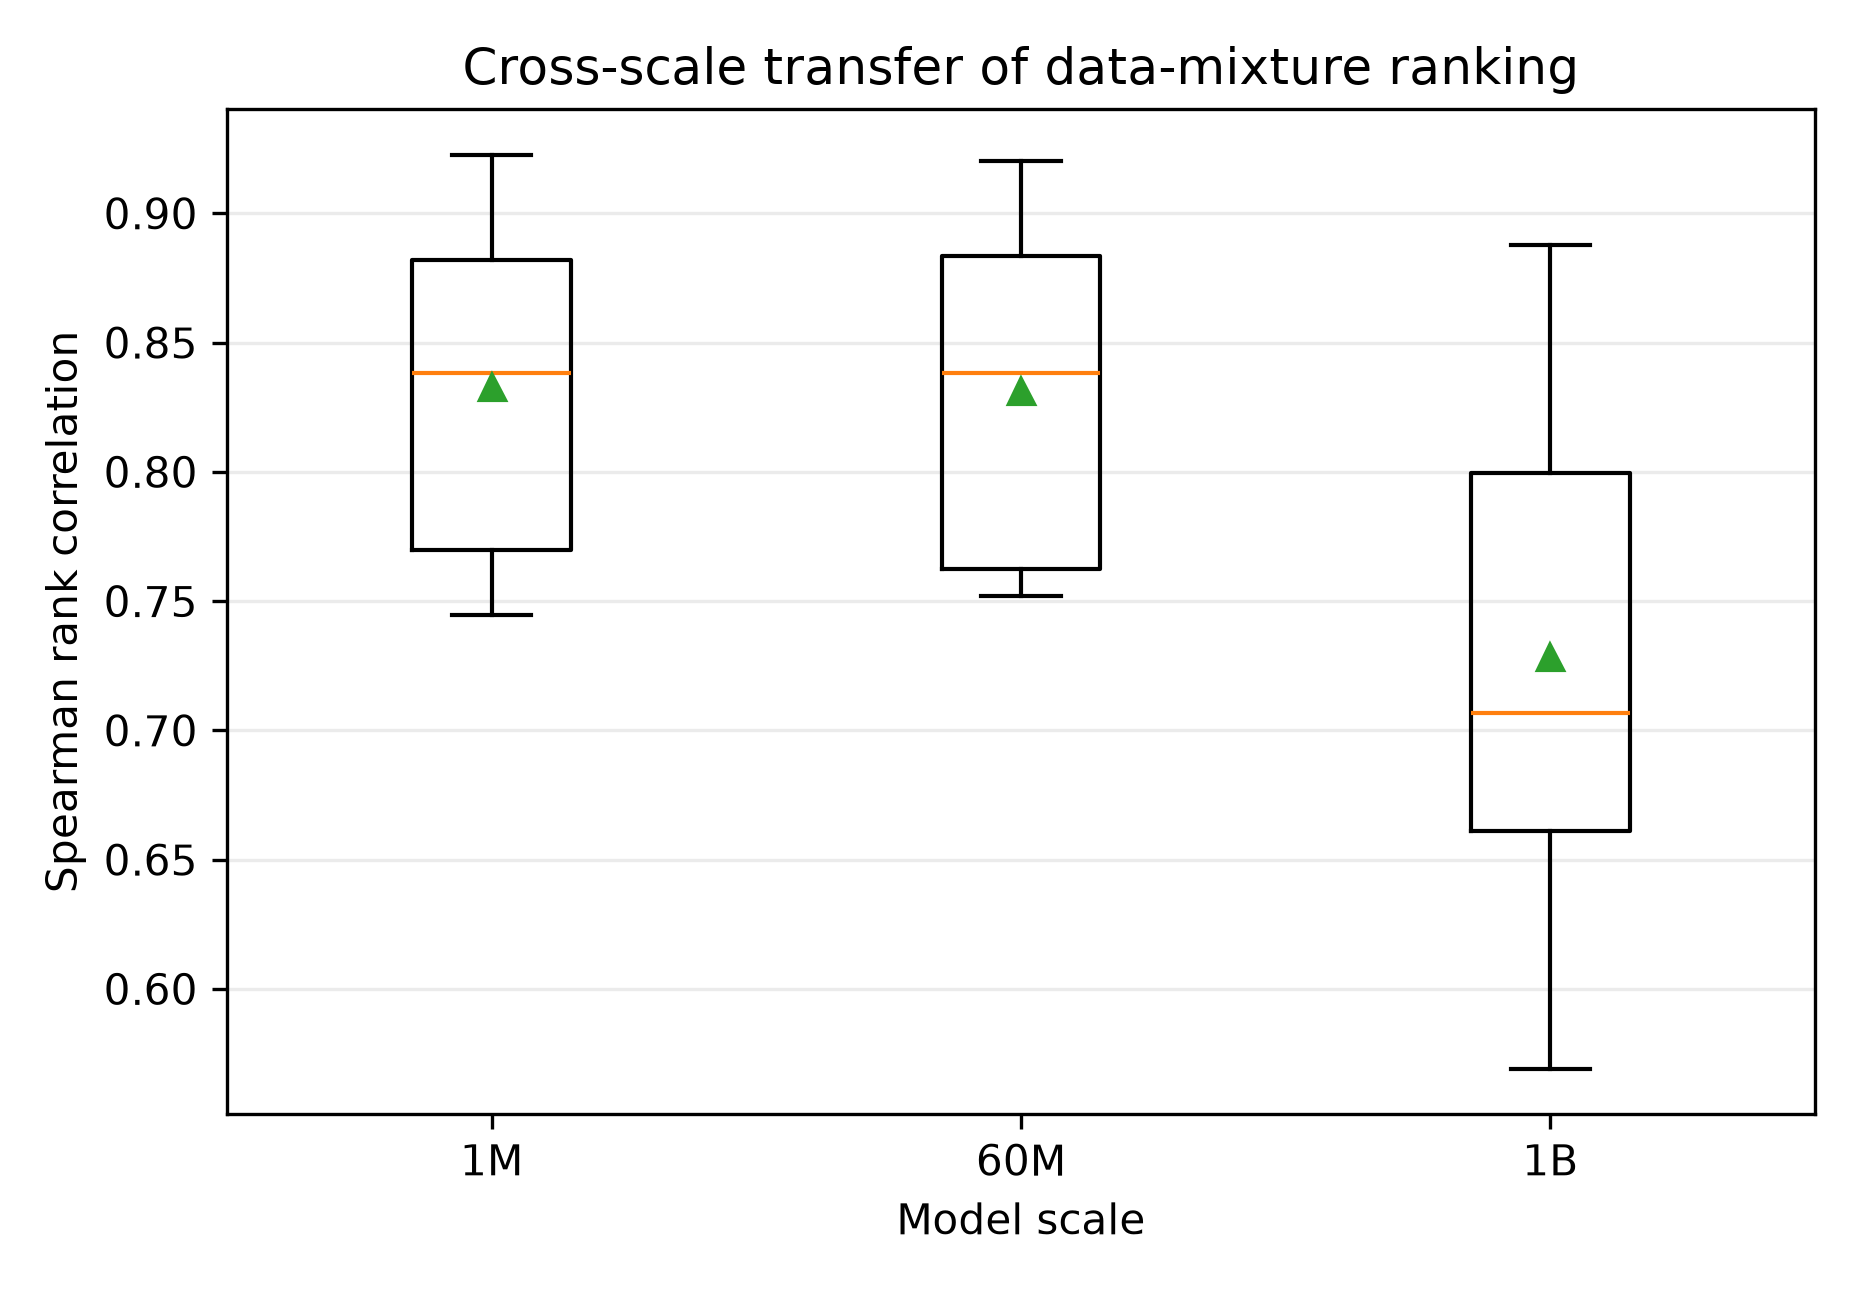
\includegraphics[width=.82\linewidth]{q1_domainwise_spearman_box.png}
\caption{冻结的 1M Ridge 代理在三个真实检验组上的逐目标域排序表现。1B 使用不同的配方集合，因此其变化不能解释为纯参数规模效应。}
\label{fig:q1_rank}
\end{figure}

A6 与 A8 使用完全相同的 256 条配方，因此还可以不依赖任何代理，直接比较两个实验组的真实 Loss 排序：
\begin{equation}
\rho_{k}^{1M\leftrightarrow 60M}
=
\rho_{\mathrm S}
\left(
L_{k}^{1M}(\boldsymbol p_i),
L_{k}^{60M}(\boldsymbol p_i)
\right).
\label{eq:q1_direct_rank}
\end{equation}
13 个目标域的相关范围为 0.9801--0.9980，中位数为 0.9944，见图\ref{fig:q1_direct_rank}。这只能说明在题目给定的这两组实验条件下，同一批配方的相对优劣高度稳定；由于 A 数据没有对应的 $D$ 等训练控制变量，本文不把这种差异单独归因于参数量 $N$。

\begin{figure}[htbp]
\centering
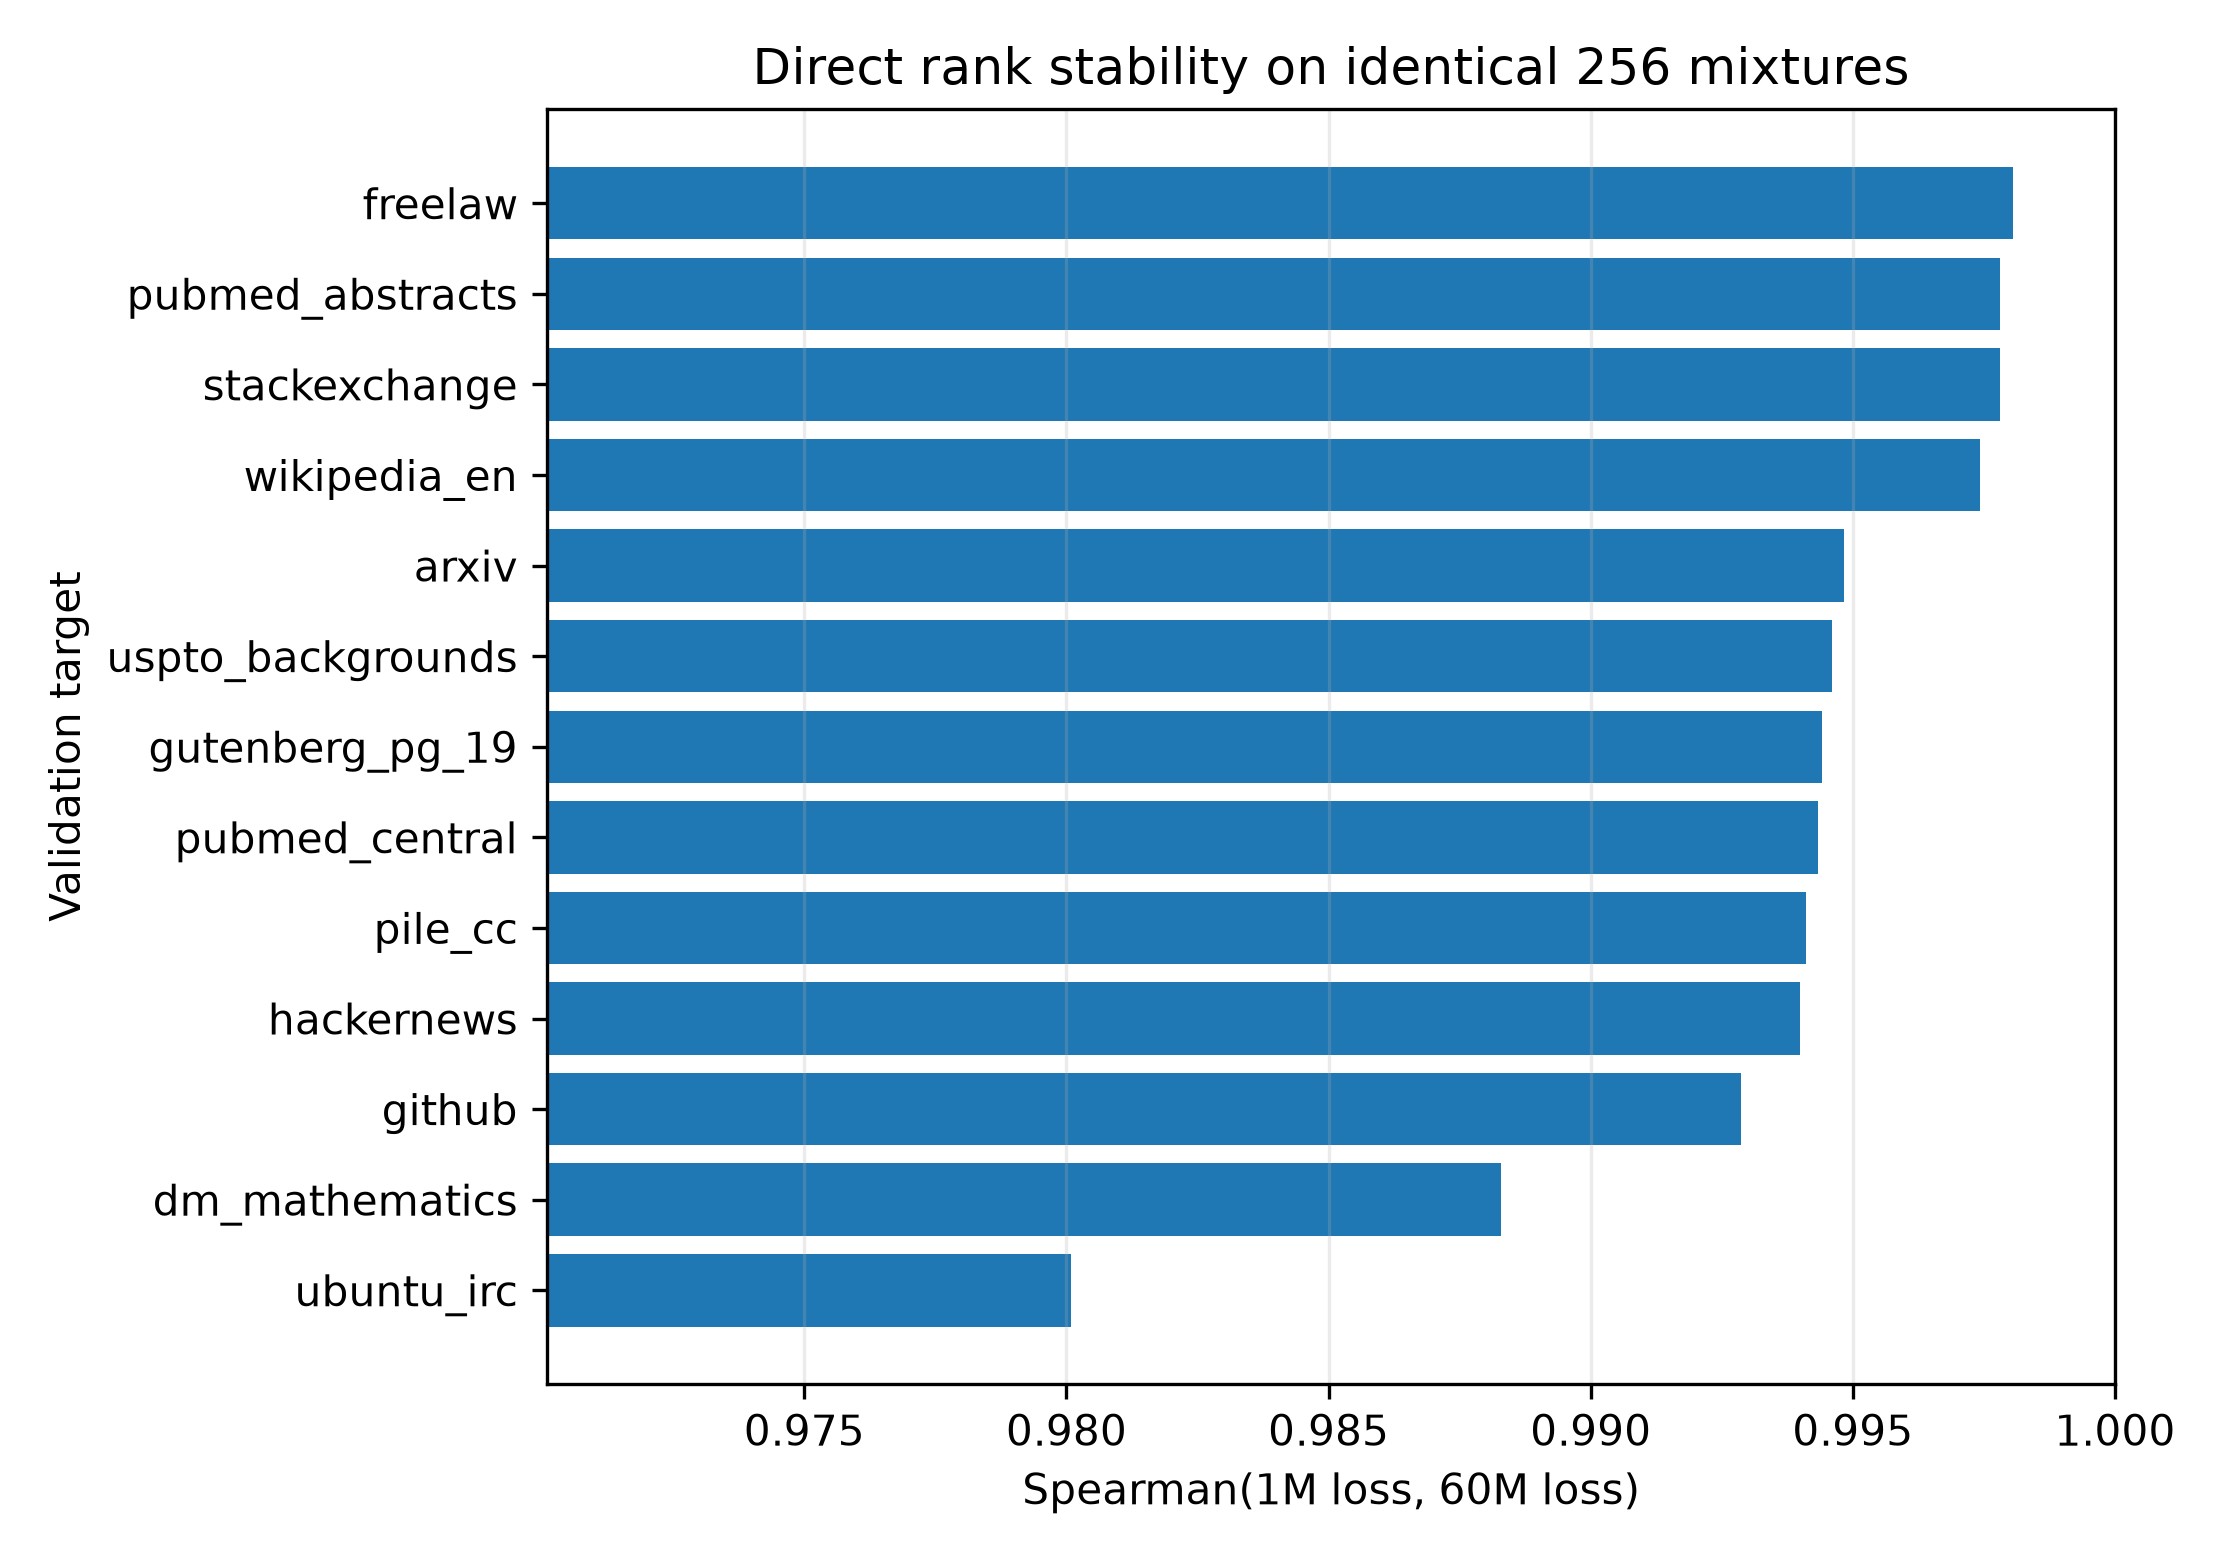
\includegraphics[width=.82\linewidth]{q1_direct_rank_stability_1m_60m.png}
\caption{相同 256 条配方在 1M 与 60M 两个真实实验组中的 Loss 排序稳定性。}
\label{fig:q1_direct_rank}
\end{figure}

A10 的 64 个 1B 配方与 A4/A6 的配方集合没有完全重复，因此 1B 的式\eqref{eq:q1_rank_validation}属于未见配方集合上的外部排序检验。它可以支持“1M 学到的配比排序仍保留部分信息”，但不能支持连续的 $N$ 尺度传递。

\subsubsection{绝对 Loss 迁移的反证性诊断}

若直接把 A4+A5 的 1M 代理当作其他实验组的绝对 Loss 预测器，则尺度平移会显著影响 RMSE。删除全部配比变量、只使用 A4+A5 中该目标域的常数均值作为基线时，1M、60M、1B 的 13 域 RMSE 中位数分别为 0.6759、1.4724、3.2514；完整 Ridge 分别为 0.4478、1.4450、3.2079。完整模型在 1M 和 60M 上分别有 13/13 个目标域的 RMSE 下降，但到 1B 只有 4/13 个目标域下降。

\begin{figure}[htbp]
\centering
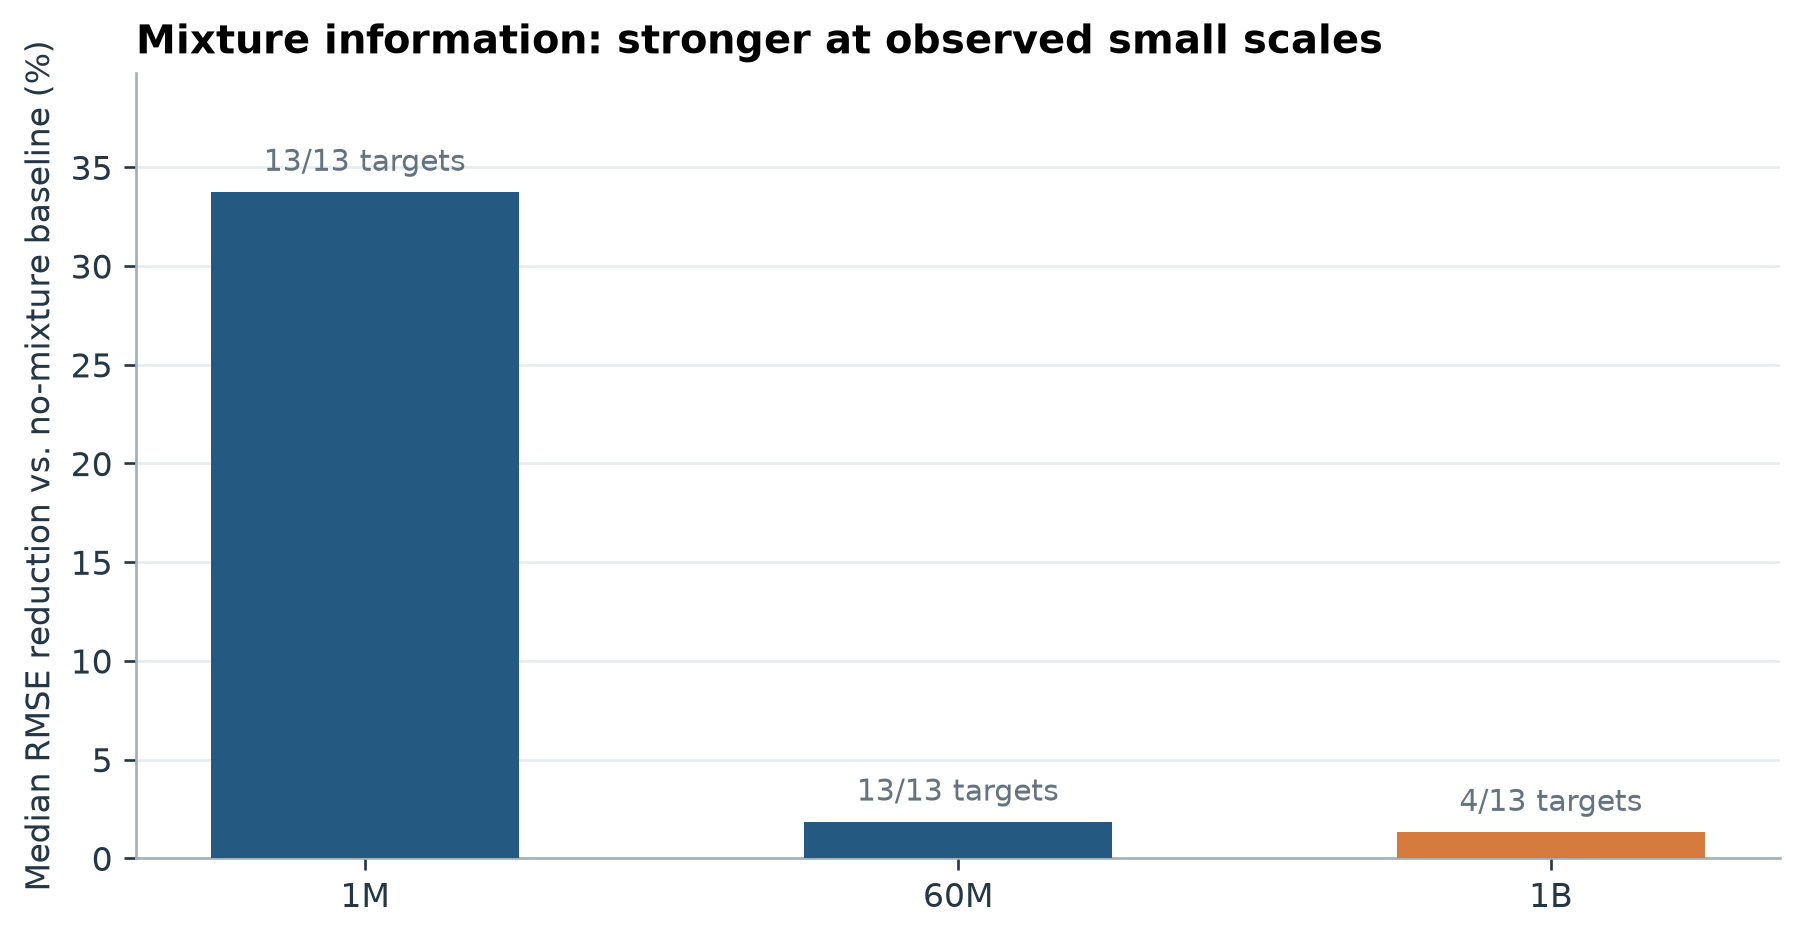
\includegraphics[width=.82\linewidth]{q1_mixture_ablation.png}
\caption{冻结 1M 配比代理相对于无配比常数基线的 RMSE 诊断。该图用于说明绝对 Loss 不能由附件 A 直接跨规模搬运，而非构造尺度律。}
\label{fig:q1_ablation}
\end{figure}

因此第一问的主要可验证结论是“配方排序具有迁移信息”，而不是“1M Loss 幅度可以按某个 $N$ 的函数外推”。原先利用三个离散实验组拟合 $b_k(N)$ 和公共衰减指数 $\eta$ 的做法不再进入主模型：A 数据既没有与配方实验对应的 $D$，又只有三个模型规模位置，且 1B 的配方支持集与 1M/60M 不同，无法把斜率变化唯一归因于 $N$。

\subsubsection{A12--A15 的使用边界}

A12--A15 的 10B/70B Loss 在数据说明中明确标记为 estimated/extrapolated，因此既不参与 Ridge 拟合，也不参与模型选择。两组使用相同的 63 个配方，且这 63 个配方均已出现在 A4 的 1M 训练配方集合中。附件给出的 10B 与 70B estimated Loss 在 13 个目标域中的直接 Spearman 范围为 0.9754--0.9965，中位数 0.9907；但冻结的 1M Ridge 在这两组 estimated Loss 上的 13 域 Spearman 中位数仅为 0.5136 和 0.4148。故 A12--A15 只作为附件内部的外推压力测试，不能作为真实大模型训练验证，也不能补足连续尺度识别。

\subsection{Q1 向后续问题的严格接口}

A16 中仅有 3 个 direct、3 个 near-direct 域映射，其余 11 个为 inferred，因此本文不生成 17 个看似精确的质量真值。第一问正式交付如下：

\begin{enumerate}
  \item 七个质量域的 A 侧综合质量代理 $Q_A$、条件抽样区间及评分规则敏感性。$Q_A$ 是描述性复合指标，不等于附件 B6--B8 的原生 $Q_{\mathrm{score}}$。
  \item 17 维配比的 13 个目标域 1M Ridge 代理，以及式\eqref{eq:q1_centered_effect}定义的 target-specific 相对配比效应 $m_k(\boldsymbol p)$。
  \item A6--A11 给出的跨实验组排序验证和 A12--A15 的 estimated/extrapolated 压力测试。
\end{enumerate}

附件 A 没有提供 $Q_A\leftrightarrow Q_{\mathrm{score}}$ 的成对标定样本，也没有证明任一 Q1 目标域 Loss 与 B1 的 \texttt{val\_loss} 属于同一数值坐标。因此第一问不提供 $Q_A\to Q_{\mathrm{score}}$ 的数值映射，不把 $m_k(\boldsymbol p)$ 直接加到 B1 Loss，也不提供由 A 数据拟合的 $\eta$、$b_k(N)$ 或其他连续尺度传递参数。$N$、$D$、B-native $Q$ 与 Loss 的统一关系由问题二依据附件 B 独立建立；若后续需要把 $m_k(\boldsymbol p)$ 映射到 B 侧 Loss，必须额外给出可验证的 Loss 坐标桥接证据。

\subsection{本问结论与局限}

在题目附件能够直接识别的范围内，问题一得到三点结论。第一，22 维质量信号可以构造透明的 A 侧综合质量代理，但其数值依赖明确的方向和权重假设，不能解释为客观质量真值；A2/A3 的非重叠记录支持 arxiv/github 域级结论在扩展样本上的稳定性。第二，A4+A5 的逐目标域 Ridge 能在 held-out 1M、60M 和 1B 配方上保持明显的排序信息，其中 1M/60M 同配方真实 Loss 的中位 Spearman 为 0.9944。第三，绝对 Loss 的跨实验组误差和 1B 支持集变化表明，附件 A 不足以单独建立连续的配比尺度律。

因此，本问只输出“质量代理、配比相对效应、排序验证和映射边界”，把 $N$、$D$ 与 B-native 质量坐标上的广义 Loss 建模严格留给问题二，从而使四问之间的递进关系与题目提供的数据保持一致。


\bibliographystyle{gmcm}
\bibliography{references}
\end{document}
